\documentclass{article}
\usepackage{amsmath}
\usepackage{hyperref}
\usepackage{graphicx}
\usepackage{float}
\usepackage[a4paper, margin=1in]{geometry}
\begin{document}

% ROS 2 Robotics Training Module: Navigation and Localization with RTAB-Map

% Introduction

\section*{Modul Pelatihan Teaching Factory Programming: Navigasi dan Lokalisasi dengan RTAB-Map}
Program pelatihan ini dirancang untuk mahasiswa yang sudah memiliki pengetahuan dasar tentang ROS2.
Fokus pelatihan adalah pada navigasi, lokalisasi, navigasi waypoint, dan pengendalian misi menggunakan state machine.
Pelatihan ini menggunakan simulasi TurtleBot dan RTAB-Map.

% Module 1
\section{Modul 1: Setup \& Installasi}

\subsection{Konfigurasi Environment}
\begin{itemize}
  \item Install ROS 2 Humble
        lakukan installasi menggunakan \href{https://docs.ros.org/en/humble/Installation/Ubuntu-Install-Debs.html}{\textbf{panduan instalasi Debian}}
  \item Install TurtleBot3 packages menggunakan \href{https://emanual.robotis.com/docs/en/platform/turtlebot3/quick-start/#installing-turtlebot3-packages}{\textbf{panduan instalasi TurtleBot3}}
  \item Install Gazebo dengan \texttt{sudo apt install ros-humble-desktop}
  \item Install RViz2 dengan \texttt{sudo apt install ros-humble-rviz2}
  \item Install RTAB-Map dengan \texttt{sudo apt install ros-humble-rtabmap-ros}
  \item Install Navigation2 dengan \texttt{sudo apt install ros-humble-navigation2 ros-humble-nav2-bringup}
\end{itemize}

\subsection{Menjalankan Simulasi}
Setelah semua paket terinstal, jalankan simulasi TurtleBot3 Waffle Pi di Gazebo dengan environment \texttt{house}:
\begin{verbatim}
export TURTLEBOT3_MODEL=waffle_pi
ros2 launch turtlebot3_gazebo turtlebot3_house.launch.py
\end{verbatim}

\subsection{Teleoperation}
Buka terminal lain untuk menjalankan teleop:
\begin{verbatim}
ros2 run turtlebot3_teleop teleop_keyboard
\end{verbatim}

\subsection{RViz2}
Buka RViz2 untuk melihat topik yang dipublish dan TF yang dimiliki robot:
\begin{verbatim}
rviz2
\end{verbatim}
Atur Fixed Frame ke \texttt{odom}.
Tambahkan display untuk \texttt{LaserScan}, dan \texttt{TF}.
Sehingga akan muncul tampilan seperti berikut:
\begin{figure}[H]
  \centering
  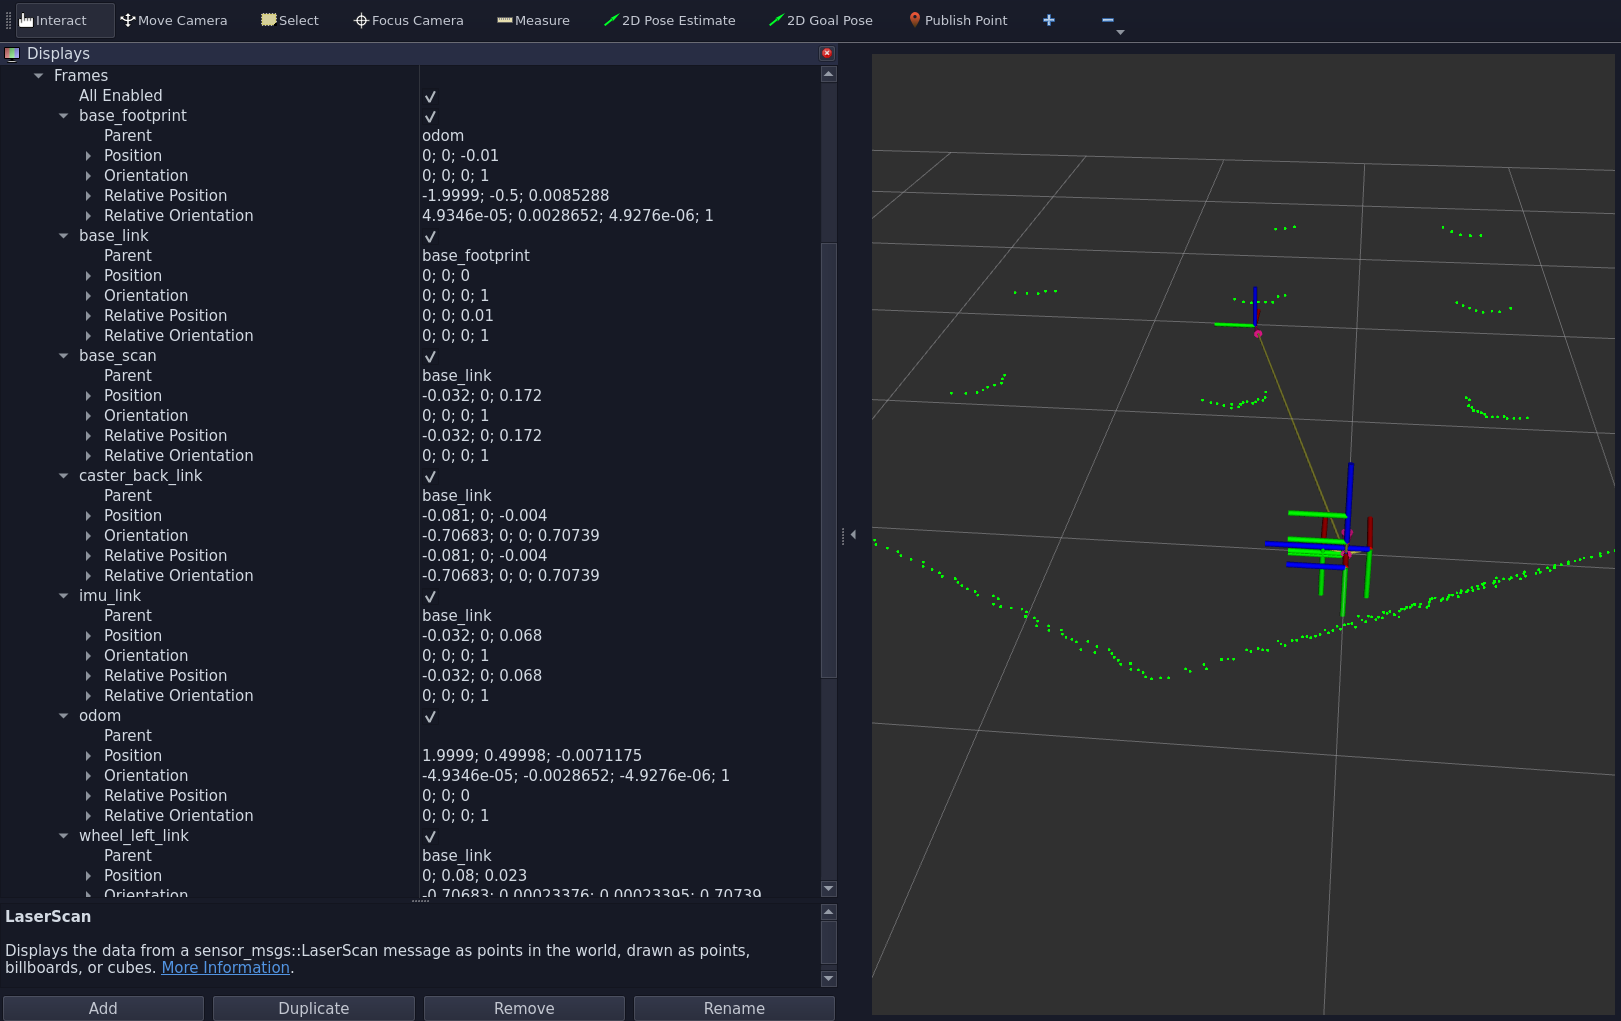
\includegraphics[width=1\textwidth]{rviz2.png}
  \caption{Contoh tampilan RViz2}
\end{figure}

Pada sidebar ditunjukkan TF yang dimiliki robot:
\begin{itemize}
  \item \texttt{odom}: frame odometri, bergerak relatif terhadap \texttt{base\_link}
  \item \texttt{base\_footprint}: frame footprint robot (sejajar dengan ground plane 2D)
  \item \texttt{base\_link}: frame utama robot (dapat mengalami translasi dan orientasi)
  \item \texttt{caster\_back\_link}: frame caster back (free wheel)
  \item \texttt{imu\_link}: frame IMU
  \item \texttt{base\_scan}: frame laser scan
  \item \texttt{wheel\_left\_link}: frame roda kiri
  \item \texttt{wheel\_right\_link}: frame roda kanan
  \item \texttt{camera\_link}: frame dasar kamera (body), menunjukkan posisi fisik kamera pada robot. Orientasi mengikuti konvensi ROS, yaitu $x$ ke depan, $y$ ke kiri, dan $z$ ke atas.
  \item \texttt{camera\_rgb\_frame}: frame kamera RGB (sensor), digunakan sebagai acuan untuk data gambar. Orientasinya sama dengan \texttt{camera\_link}.
  \item \texttt{camera\_rgb\_optical\_frame}: frame kamera dengan konvensi optik. Orientasi mengikuti standar OpenCV, yaitu $z$ ke depan, $x$ ke kanan, dan $y$ ke bawah.
\end{itemize}
Semua TF tersebut terhubung dalam sebuah pohon (tree) yang dapat dilihat pada tab \texttt{TF} di RViz2. atau dengan perintah:
\begin{verbatim}
ros2 run tf2_tools view_frames.py
\end{verbatim}
Perintah ini akan menghasilkan file \texttt{frames.pdf} yang menunjukkan struktur pohon TF sebagai berikut:
\begin{figure}[H]
  \centering
  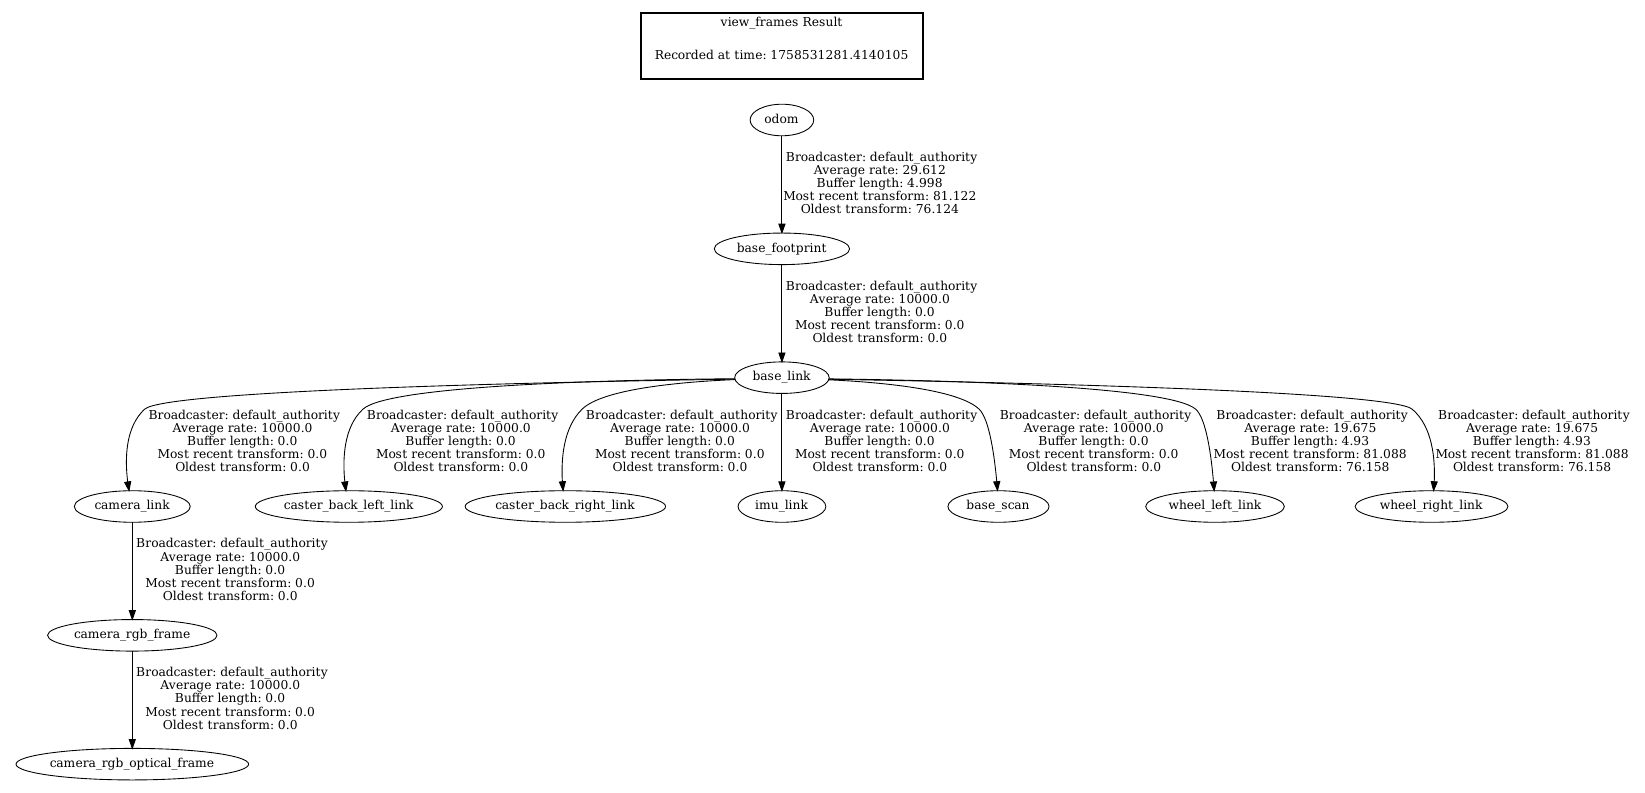
\includegraphics[width=1\textwidth]{tf_tree.png}
  \caption{Contoh TF Tree}
\end{figure}


% Module 2
\section{Modul 2: Mapping dengan RTAB-Map}
\textbf{Objectives:}
\begin{itemize}
  \item Understand SLAM and RTAB-Map
  \item Run RTAB-Map in simulation
  \item Save and load maps
\end{itemize}
\textbf{Exercises:}
\begin{itemize}
  \item Launch TurtleBot3 with RTAB-Map
  \item Explore environment to build map
  \item Save map using \texttt{ros2 run nav2\_map\_server map\_saver\_cli}
\end{itemize}

% Module 3
\section{Module 3: Localization with RTAB-Map}
\textbf{Objectives:}
\begin{itemize}
  \item Use pre-built maps for localization
  \item Understand TF tree: map $\rightarrow$ odom $\rightarrow$ base\_link
\end{itemize}
\textbf{Exercises:}
\begin{itemize}
  \item Launch localization node with map.yaml
  \item Move robot and verify pose in RViz
\end{itemize}

% Module 4
\section{Module 4: Navigation with Nav2}
\textbf{Objectives:}
\begin{itemize}
  \item Learn Navigation2 stack
  \item Configure global and local planners
  \item Tune costmap parameters
\end{itemize}
\textbf{Exercises:}
\begin{itemize}
  \item Launch nav2\_bringup with TurtleBot
  \item Send a navigation goal in RViz
  \item Observe path planning and execution
\end{itemize}

% Final Project
\section*{Final Project}
Students implement a complete mission-based program:
\begin{itemize}
  \item Explore and build map with RTAB-Map
  \item Localize using saved map
  \item Patrol using waypoints
  \item Implement mission logic with state machine
\end{itemize}

\end{document}
